\subsection{Haute disponibilité}

\begin{frame}{Haute disponibilité}

    Pour garantir qu'un service soit disponible, il existe plusieurs mécanismes :

    \begin{itemize}
        \item Redondance
        \item Réplication
        \item Répartition de la charge (\textit{load balancing})
        \item Bascule automatique (\textit{failover})
    \end{itemize}

    \note{
        \begin{itemize}
            \item \textbf{Redondance} : dupliquer les composants critiques (serveurs, bases de données, réseaux) pour qu'un élément puisse prendre le relais en cas de défaillance d'un autre
            \item \textbf{Répartition de charge} (load balancing) : distribuer le trafic entre plusieurs serveurs pour éviter qu'un seul point ne soit surchargé ou constitue un point de défaillance unique
            \item \textbf{Basculement automatique} (failover) : détecter une panne et rediriger automatiquement le trafic vers un système de secours
            \item \textbf{Réplication de données} : garder plusieurs copies synchronisées des données, souvent sur des sites géographiquement distincts
        \end{itemize}

    }

\end{frame}

\begin{frame}{Redondance}

    \begin{figure}[htb]
        \centering
        \includegraphics[width=0.9\textwidth]{img/redundancy.png}
    \end{figure}

    \note{
        La redondance consiste à dupliquer les composants critiques d'un système pour assurer la continuité de service en cas de défaillance. Cela peut inclure des serveurs, des bases de données, des réseaux, etc.

        Par exemple, si un serveur tombe en panne, un autre serveur redondant peut prendre le relais sans interruption de service. Cela permet d'améliorer la disponibilité et la fiabilité du système.
    }

\end{frame}

\begin{frame}{Réplication}

    \begin{figure}[htb]
        \centering
        \includegraphics[width=0.9\textwidth]{img/replication.png}
    \end{figure}

    \note{
        Les copies de A sont créees et stockées sur d'autres nœuds du cluster pour assurer la redondance, appelées \textbf{répliques} (ou \textit{replicas}). Cela permet de garantir la disponibilité des données même si un nœud tombe en panne.

        Il existe deux types de réplication :
        \begin{itemize}
            \item Réplication synchrone : les données sont écrites sur tous les nœuds avant de confirmer l'écriture
            \item Réplication asynchrone : les données sont écrites sur un nœud principal et répliquées sur les nœuds secondaires après coup
        \end{itemize}

        En pratique, la réplication est souvent un moyen d'implémenter la redondance au niveau des données. Un système hautement disponible combine généralement les deux :
        \begin{itemize}
            \item On a des serveurs redondants (redondance de composants)
            \item Ces serveurs contiennent chacun une copie à jour de la base de données (réplication des données)
        \end{itemize}

    }

\end{frame}

\begin{frame}{Sans load balancer}

    \begin{figure}[htb]
        \centering
        \includegraphics[width=0.9\textwidth]{img/without-load-balancing.png}
    \end{figure}

\end{frame}

\begin{frame}{Avec load balancer}

    \begin{figure}[htb]
        \centering
        \includegraphics[width=0.9\textwidth]{img/with-load-balancing.png}
    \end{figure}

\end{frame}

\begin{frame}{Failover}

    \begin{figure}[htb]
        \centering
        \includegraphics[width=0.9\textwidth]{img/cluster-failover-map.png}
    \end{figure}

    \note{
        Le failover est un mécanisme qui permet de basculer automatiquement vers un système de secours en cas de défaillance du système principal. Cela peut inclure des serveurs, des bases de données, des réseaux, etc.

        Par exemple, si un serveur tombe en panne, le trafic peut être redirigé vers un serveur de secours sans interruption de service. Cela permet d'améliorer la disponibilité et la fiabilité du système.
    }

\end{frame}
% ----------------------------------------------------------------------------------------------------------------------
% ----------------------------------------------------------------------------------------------------------------------
% ----------------------------------------------------------------------------------------------------------------------

\subsection{Théorème CAP}

\begin{frame}{Théorème CAP}

    \begin{columns}
        \begin{column}{0.5\textwidth}
            \begin{center}
             	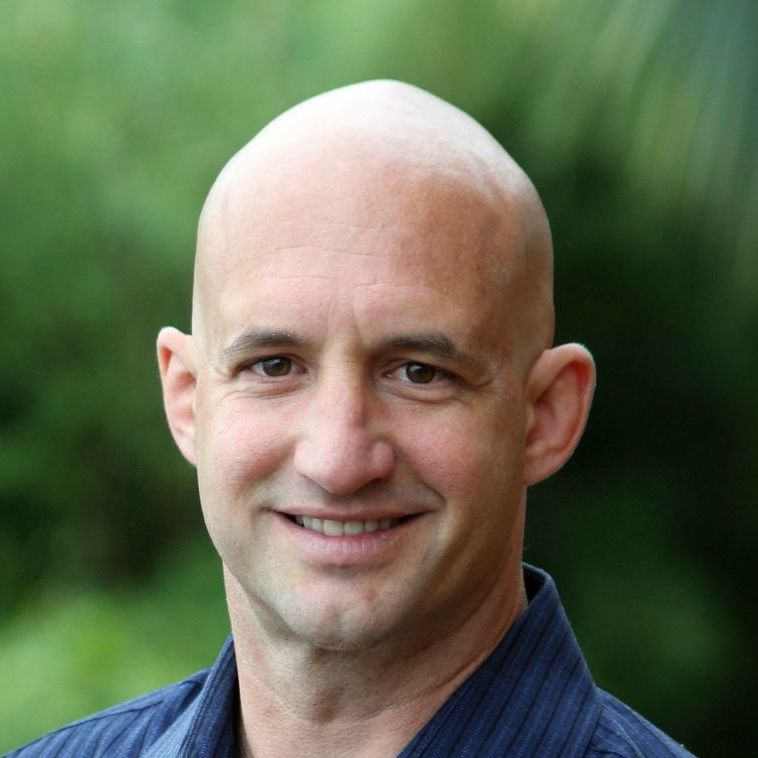
\includegraphics[width=0.7\textwidth]{img/eric-brewer.jpg}\\
             	\vspace{0.3cm}
                Eric Brewer\\
                Professeur à l'université de Berkeley
             \end{center}
        \end{column}
        \begin{column}{0.63\textwidth}
               Selon \textbf{Eric Brewer}, un système informatique ne peut pas garantir simultanément la \textcolor{color-consistency}{\bf consistance}, la \textcolor{color-availability}{\bf disponibilité} et la \textcolor{color-partition}{\bf tolérance aux partitions}. Il faut faire un compromis entre les trois propriétés.
        \end{column}
    \end{columns}

    \note{
        CAP, c’est comme choisir entre : avoir toujours la bonne info (C), toujours un service disponible (A), ou tolérer les pannes (P).
    }


\end{frame}

\begin{frame}{Mais que signifie le théorème CAP ?}
    \begin{itemize}
        \item \textcolor{color-consistency}{\bf Consistency} : toutes les données sont à jour
        \pause
        \item \textcolor{color-availability}{\bf Availability} : toutes les requêtes reçoivent une réponse
        \pause
        \item \textcolor{color-partition}{\bf Partition tolerance} : le système continue de fonctionner malgré les défaillances réseau
    \end{itemize}

    \note{
        \textcolor{color-consistency}{\bf Consistency} : toutes les copies des données sont identiques et à jour. Si une donnée est modifiée, toutes les répliques doivent refléter ce changement immédiatement.

        Un système est cohérent si le client peut interroger n’importe quelle réplique d’un objet à un instant donné, et obtenir à chaque fois le même résultat.

        Pour des raisons d’efficacité, les systèmes distribuées créent et propagent les répliques de manière asynchrone. Il est donc possible qu’un objet ne soit pas cohérent pendant un court instant, le temps que les répliques se fassent.

        De nombreux systèmes \textbf{garantissent ainsi une cohérence à terme} (eventual consistency).


        \textcolor{color-availability}{\bf Availability} : le système répond toujours aux requêtes, même si certaines parties du système sont en panne. Chaque requête reçoit une réponse, mais pas nécessairement la plus récente.

        Un système est disponible à un instant donné si toute requête envoyée au cluster par un client à ce moment est prise en compte. Cela ne signifie pas que la requête est exécutée : elle peut être mise en attente, mais le client sera au moins informé de la prise en compte.

        Mesure de la disponibilité en \%, par exemple avec une \textbf{disponibilité de 99.99\%} : système indisponible pendant au plus 0.01\% du temps. \textbf{Sur un an, cela représente un total cumulé de 53 min.}

        \textcolor{color-partition}{\bf Partition tolerance} : le système continue de \textbf{fonctionner correctement même si des messages sont perdus ou retardés} entre les nœuds du système. Il peut y avoir des partitions réseau, mais le système doit rester opérationnel.

        Par exemple, lorsqu’un nœud du cluster crashe, ou qu’un lien réseau disparaît, mettant une portion entière du cluster hors de portée.

    }

\end{frame}

\begin{frame}{Théorème CAP}

    \begin{figure}[htb]
        \resizebox{!}{0.85\textheight}{
        \begin{tikzpicture}
            % Circle 1: Consistency
            \draw[very thick, color=color-consistency, pattern=north east lines, pattern color=color-consistency] (0,0) circle (3cm);
            \node[fill=color-consistency, text=white, font=\bfseries, rounded corners] at (0,0.5) {Consistency};

            % Circle 2: Availability
            % \fill[pattern=north lines, pattern color=color-availability] (-2.5,-3.25) circle (3cm);
            \draw[very thick, color=color-availability] (-2.1,-3.25) circle (3cm);
            \node[fill=color-availability, text=white, font=\bfseries, rounded corners] at (-2.75,-3.5) {Availability};

            % Circle 3: Partition Tolerance
            % \fill[pattern=north east lines, pattern color=color-partition] (2.5,-3.25) circle (3cm);
            \draw[very thick, color=color-partition] (2.1,-3.25) circle (3cm);
            \node[fill=color-partition, text=white, font=\bfseries, rounded corners, align=left] at (2.75,-3.5) {Partition \\ tolerance};

			\onslide<2->{
	            \node[fill=none, font=\bfseries, text=color-ca] at (-1.4,-1.5) {CA};
	            \node[fill=none, font=\bfseries, text=color-cp] at (1.4,-1.5) {CP};
	            \node[fill=none, font=\bfseries, text=color-ap] at (0,-3.7) {AP};
			}
            \onslide<3->{
                \node[inner sep=0pt] (unicorn) at (0,-2.25) {
\includegraphics[width=1cm]{img/unicorn.png}};
            }
        \end{tikzpicture}
        }
    \end{figure}

    \note{

        \textbf{CA} : un problème sur un des noeuds fait stopper le système

        \textbf{CP} : les données ne sont pas forcément disponibles au moment de la requête

        \textbf{AP} : les données renvoyées ne sont pas toujours cohérentes
    }
\end{frame}
